\chapter{Results and Discussion} 
\label{chp:results}
In this section we will present the results of the models and discuss their implications.





\section{Test Dataset Results}
\begin{itemize}
    \item Discuss the data splits
    \item The number of RfAs and votes in each split
\end{itemize}

\begin{table}
    \centering
    \caption{Results of different models for the test split of the \wikirfa dataset}
    \label{tab:test-results}
    \begin{tabular}{lccc}
        \toprule
        Model & AUC-ROC & \aucposPR  & \aucnegPR \\ 
        \midrule
        
        Baseline & 0.5 & 0.776 & 0.224 \\
        \midrule

        {\shortstack[l]{Graph\\ Combination}} &  0.542 & 0.798 & 0.251 \\
        \midrule

        {\shortstack[l]{Iterative\\ Balance}} &  0.815 & 0.922 & 0.614 \\
        \midrule

        {\shortstack[l]{Iterative\\ Status}} & 0.754 & 0.9 & 0.486 \\
        
        \bottomrule
        \end{tabular}
\end{table}

\subsection{Graph Combination Model results}

\begin{figure}[htp]
    \centering
    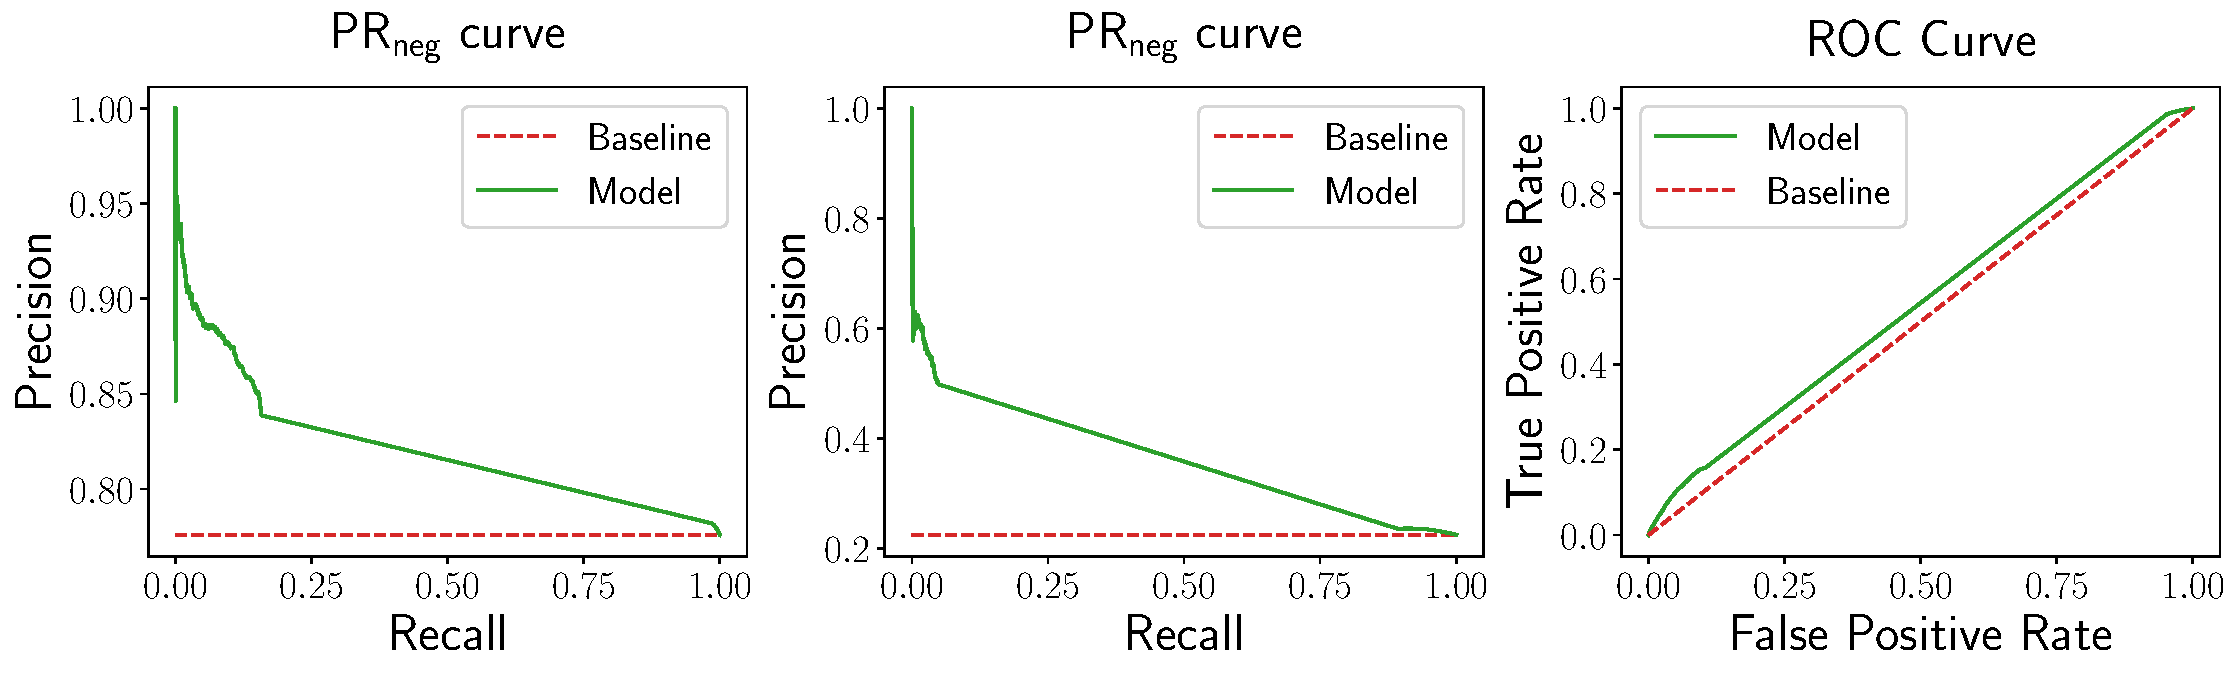
\includegraphics[width=\textwidth]{images/Logisitc Regression_test.pdf}
    \caption{Logistic Regression plots for test data}
    \label{fig:lr-test-plots}
\end{figure}

\begin{figure}[htp]
    \centering
    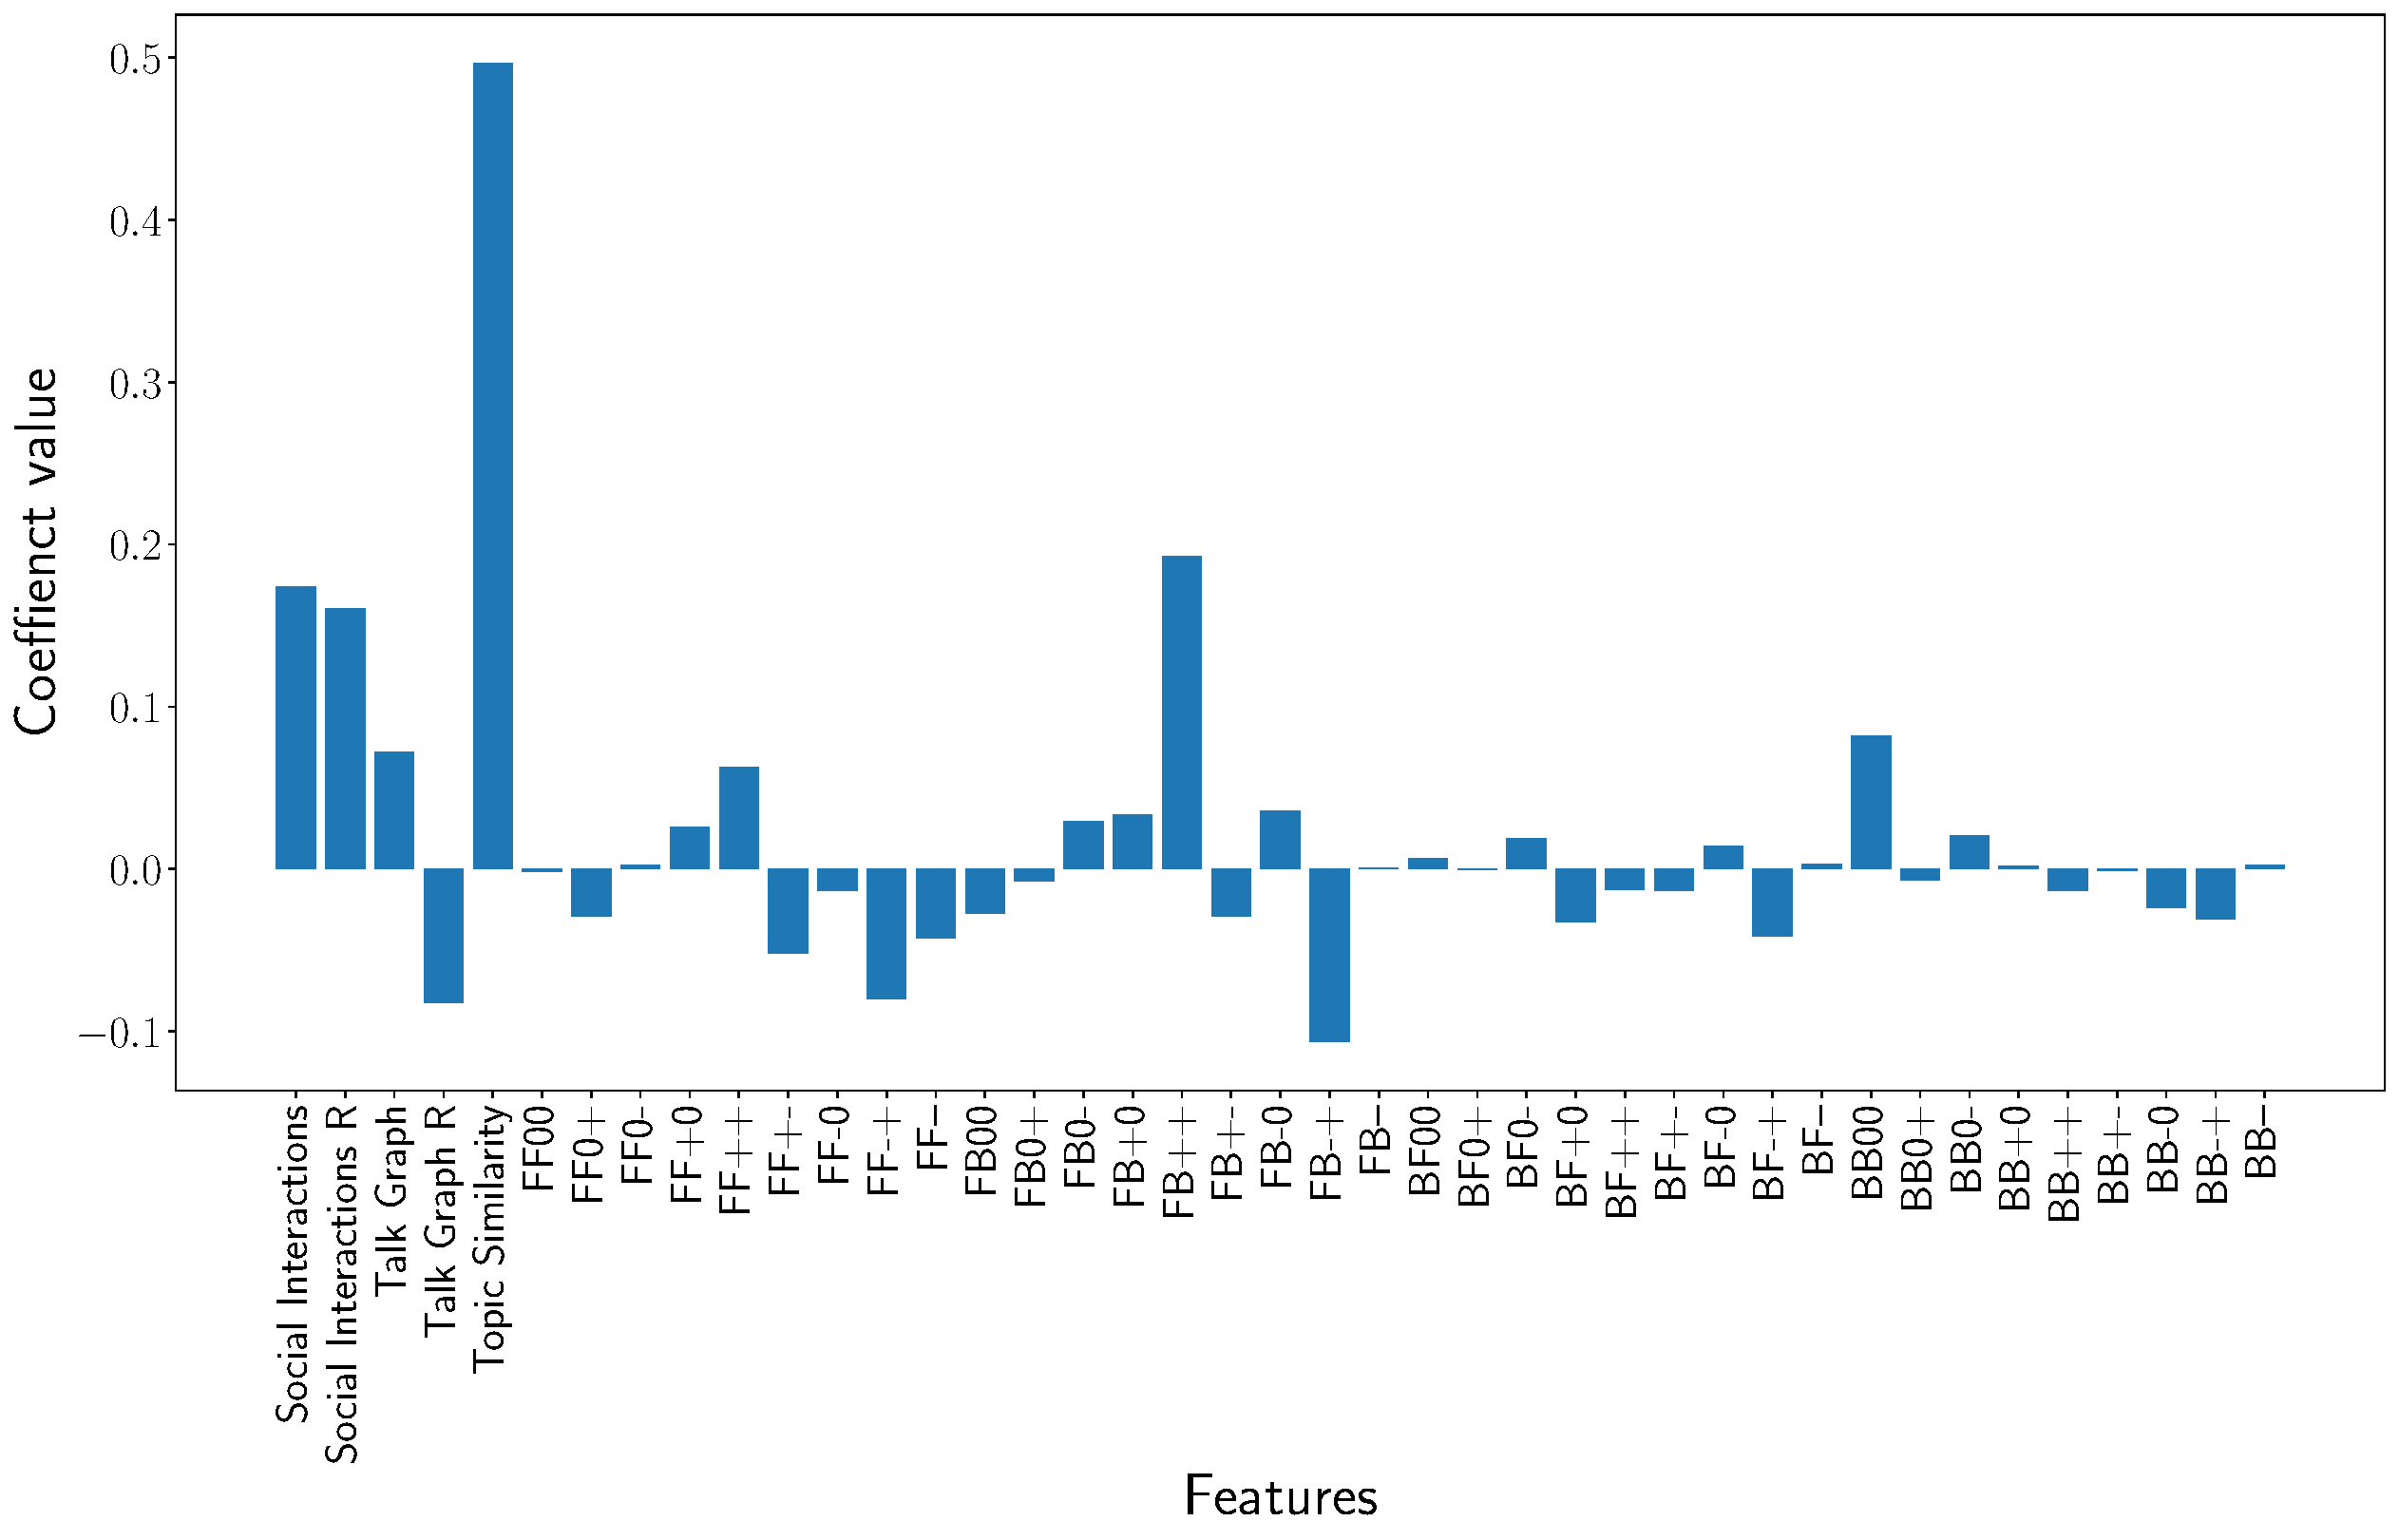
\includegraphics[width=\textwidth]{images/Logistic Regression_features.pdf}
    \caption{Feature importances for Logistic Regression model }
    \label{fig:lr-feature-importances}
\end{figure}
\begin{itemize}
    \item the description of the auxiliary graphs 
    \item Present results for LR model
    \item Show the ROC and PR curves
    \item Show the feature importances and discuss their relevance 
    \item Highlight the difficulty of predicting negative votes
\end{itemize}

\subsection{Iterative Model Results}
\begin{itemize}
    \item discuss how to compare the iterative model results
    \item Provide plots and table 
    \item Discuss the predictive power of the iterative model over the combination model
    \item Limitations and expansion of the graph combination model
\end{itemize}

\section{Complete \wikirfa Results}
\begin{table}
    \centering
    \caption{Results of iterative models on the complete \wikirfa dataset}
    \label{tab:complete-results}
    \begin{tabular}{lccc}
        \toprule
        Model & AUC-ROC & \aucposPR  & \aucnegPR \\ 
        \midrule
        
        Baseline & 0.5 & 0.784& 0.216 \\
        \midrule

        {\shortstack[l]{Iterative\\ Balance}} &  0.835 & 0.935 & 0.635 \\
        \midrule

        {\shortstack[l]{Iterative\\ Status}} & 0.784 & 0.917 & 0.502 \\
        
        \bottomrule
        \end{tabular}
\end{table}

\begin{figure}[htp]
    \centering
    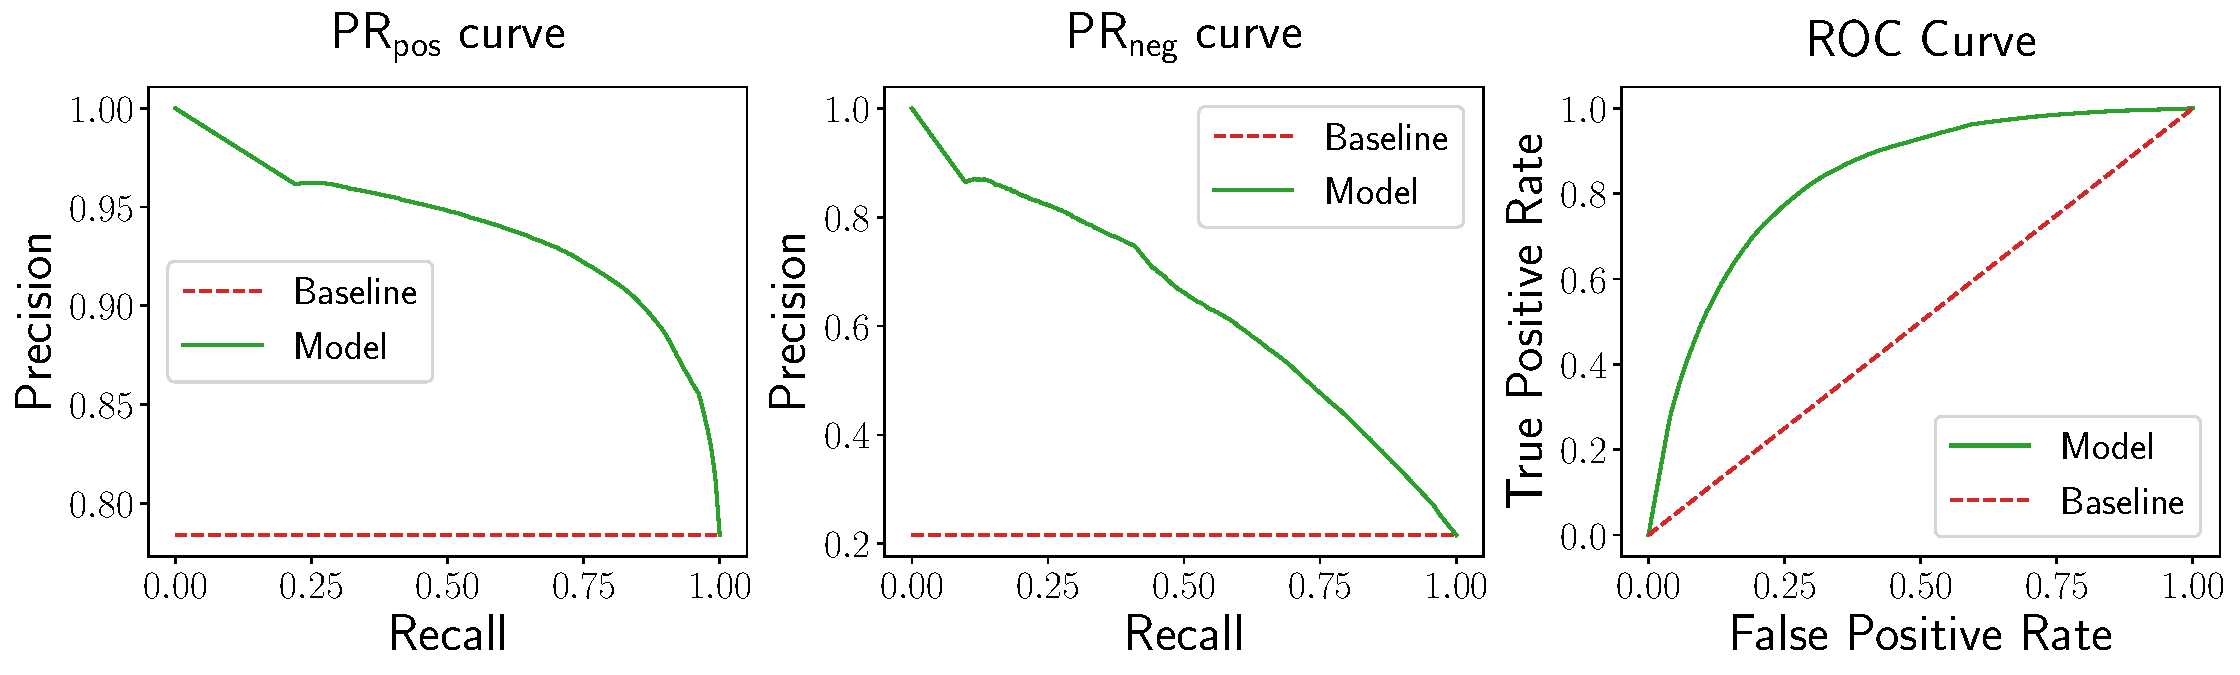
\includegraphics[width=\textwidth]{images/iterative_Balance.pdf}
    \caption{Plots for the Iterative Balance Model on the complete \wikirfa dataset}
    \label{fig:complete-iterative-balane}
\end{figure}

\begin{figure}[htp]
    \centering
    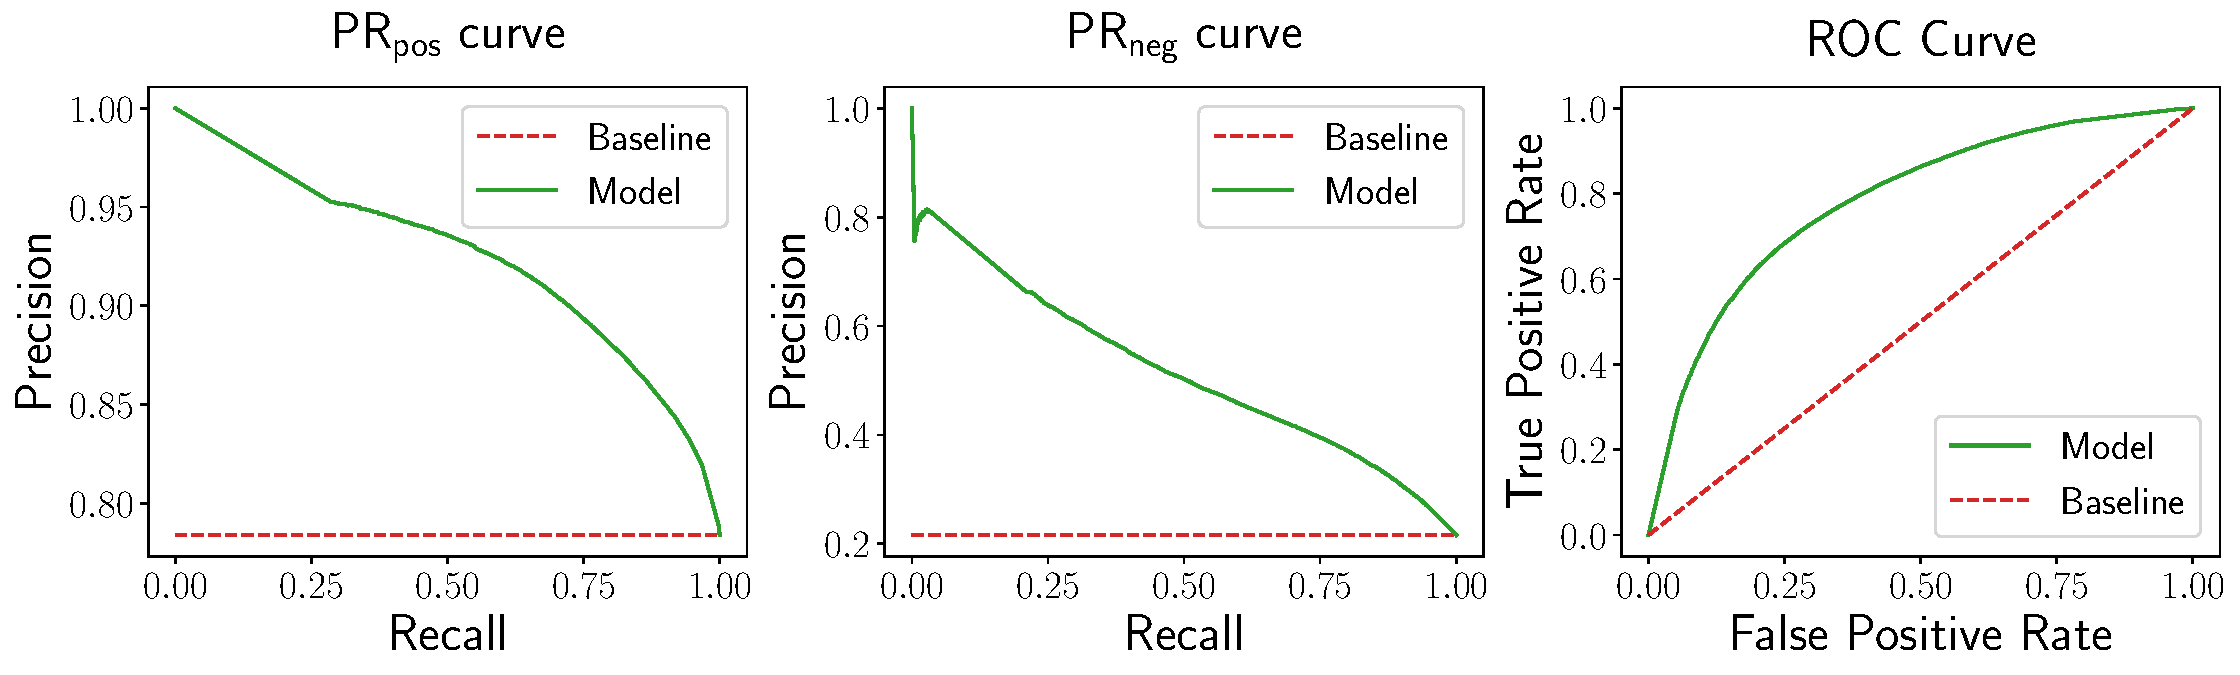
\includegraphics[width=\textwidth]{images/iterative_Status.pdf}
    \caption{Plots for the Iterative Status Model on the complete \wikirfa dataset}
    \label{fig:complete-iterative-status}
\end{figure}



\begin{itemize}
    \item Present the Iterative Balance model results
    \item Discuss quality of predictions using evaluation metrics
    \item Explain the Iterative Status model results 
    \item Explain the selection of threshold and F1-score
\end{itemize}

\section{Voting Order Results}
\begin{table}
    \centering
    \caption{Results for different vote orderings for the failed RfA}
    \label{tab:fail-rfa}
    \begin{tabular}{llccc}
        \toprule
        Model & Vote Order & AUC-ROC & \aucposPR  & \aucnegPR \\ 
        \midrule
        
        Baseline & - & 0.5 & 0.52 & 0.479 \\
        \midrule
        
        \multirow{3}{*}{\shortstack[l]{Iterative\\ Balance}} & 
        Normal &  0.543 & 0.74 & 0.454 \\
        \cmidrule{2-5}
        &Reversed & 0.74 & 0.868 & 0.572 \\
        \cmidrule{2-5}
        & Random & 0.68 & 0.812 & 0.575 \\
        \midrule

        \multirow{3}{*}{\shortstack[l]{Iterative\\ Status}} & 
        Normal & 0.962 & 0.977 & 0.909 \\
        \cmidrule{2-5}
        & Reversed & 0.930 & 0.965 & 0.806   \\
        \cmidrule{2-5}
        & Random & 0.924 & 0.957 & 0.818 \\
        \bottomrule
        \end{tabular}
\end{table}

\begin{table}
    \centering
    \caption{Results for different vote orderings for the successful RfA}
    \label{tab:pass-rfa}
    \begin{tabular}{llccc}
        \toprule
        Model & Vote Order & ROC AUC & PR Positive  & Pr Negative \\ \midrule
        Baseline & - & 0.5 & 0.905 & 0.095 \\
        \midrule
        
        \multirow{3}{*}{\shortstack[l]{Iterative\\ Balance}} & 
        Normal &  0.9175 & 0.991 & 0.385 \\
        \cmidrule{2-5}
        &Reversed & 0.720 & 0.972 & 0.142 \\
        \cmidrule{2-5}
        & Random & 0.894 & 0.989 & 0.431 \\
        \midrule
        
        \multirow{3}{*}{\shortstack[l]{Iterative\\ Status}} & 
        Normal & 0.846 & 0.981 & 0.293 \\
        \cmidrule{2-5}
        & Reversed & 0.895 & 0.99 & 0.29 \\
        \cmidrule{2-5}
        & Random & 0.931 & 0.992 & 0.451 \\
        \bottomrule
        \end{tabular}
\end{table}


